\section{Problem Statement}
\label{sec:problemStatement}

In this section, we motivate our work in the context of ensuring the integrity and confidentiality of user's IO data to/from remote servers. We also describe selected existing research works that tackle the relevant problem, and we discuss how those works lack a proper solution. Lastly, we present the goals of \name that we derive from the drawbacks of existing literature.

\subsection{Motivation: Secure IO with Remote Safety-critical System}

A user communicates with a remote server through a \emph{host} system that is typically a standard PC, which gives the host access to the raw IO data that is exchanged between the user and the remote server. The host consists of large and complex system softwares such as the operating system, device drivers, applications such as browser, and a diverse set of hardware components that expose the host to a large attack surface. An adversary that controls the user's host can alter user intentions, i.e., it can perform arbitrary actions on behalf of the user, modify the input parameters, or show wrong information to the user. Such an adversary is very powerful and difficult to be detected or prevented by a remote server. The consequences of such attacks might be severe when applications that control remote safety-critical systems are targeted. The attacker can pass the wrong input to a remote safety-critical system such as a medical device, power plant, etc.

Trusted execution environments (TEEs) enable remote trust into the code executing on the processor, effectively eliminating the need to trust more significant code base (motherboard, memory modules, OS, and other applications). Processor TEEs such as Intel SGX rely on the OS to mediate all user IO operations. Hence, the problem of isolating user's input and output remains \emph{challenging}. Therefore, service providers typically operate with the assumption that the data they receive is genuine (generated by the user) and not altered by a compromised host, or require a second device to confirm the input. System-level TEEs such as ARM TrustZone that allow the execution of IO drivers as privileged code avoid the necessity to trust the vulnerable OS. However, such a mechanism is limited to ARM platforms, making them infeasible for \emph{x86} platforms, which support TEEs like SGX. 

\begin{figure}[t]
\centering
%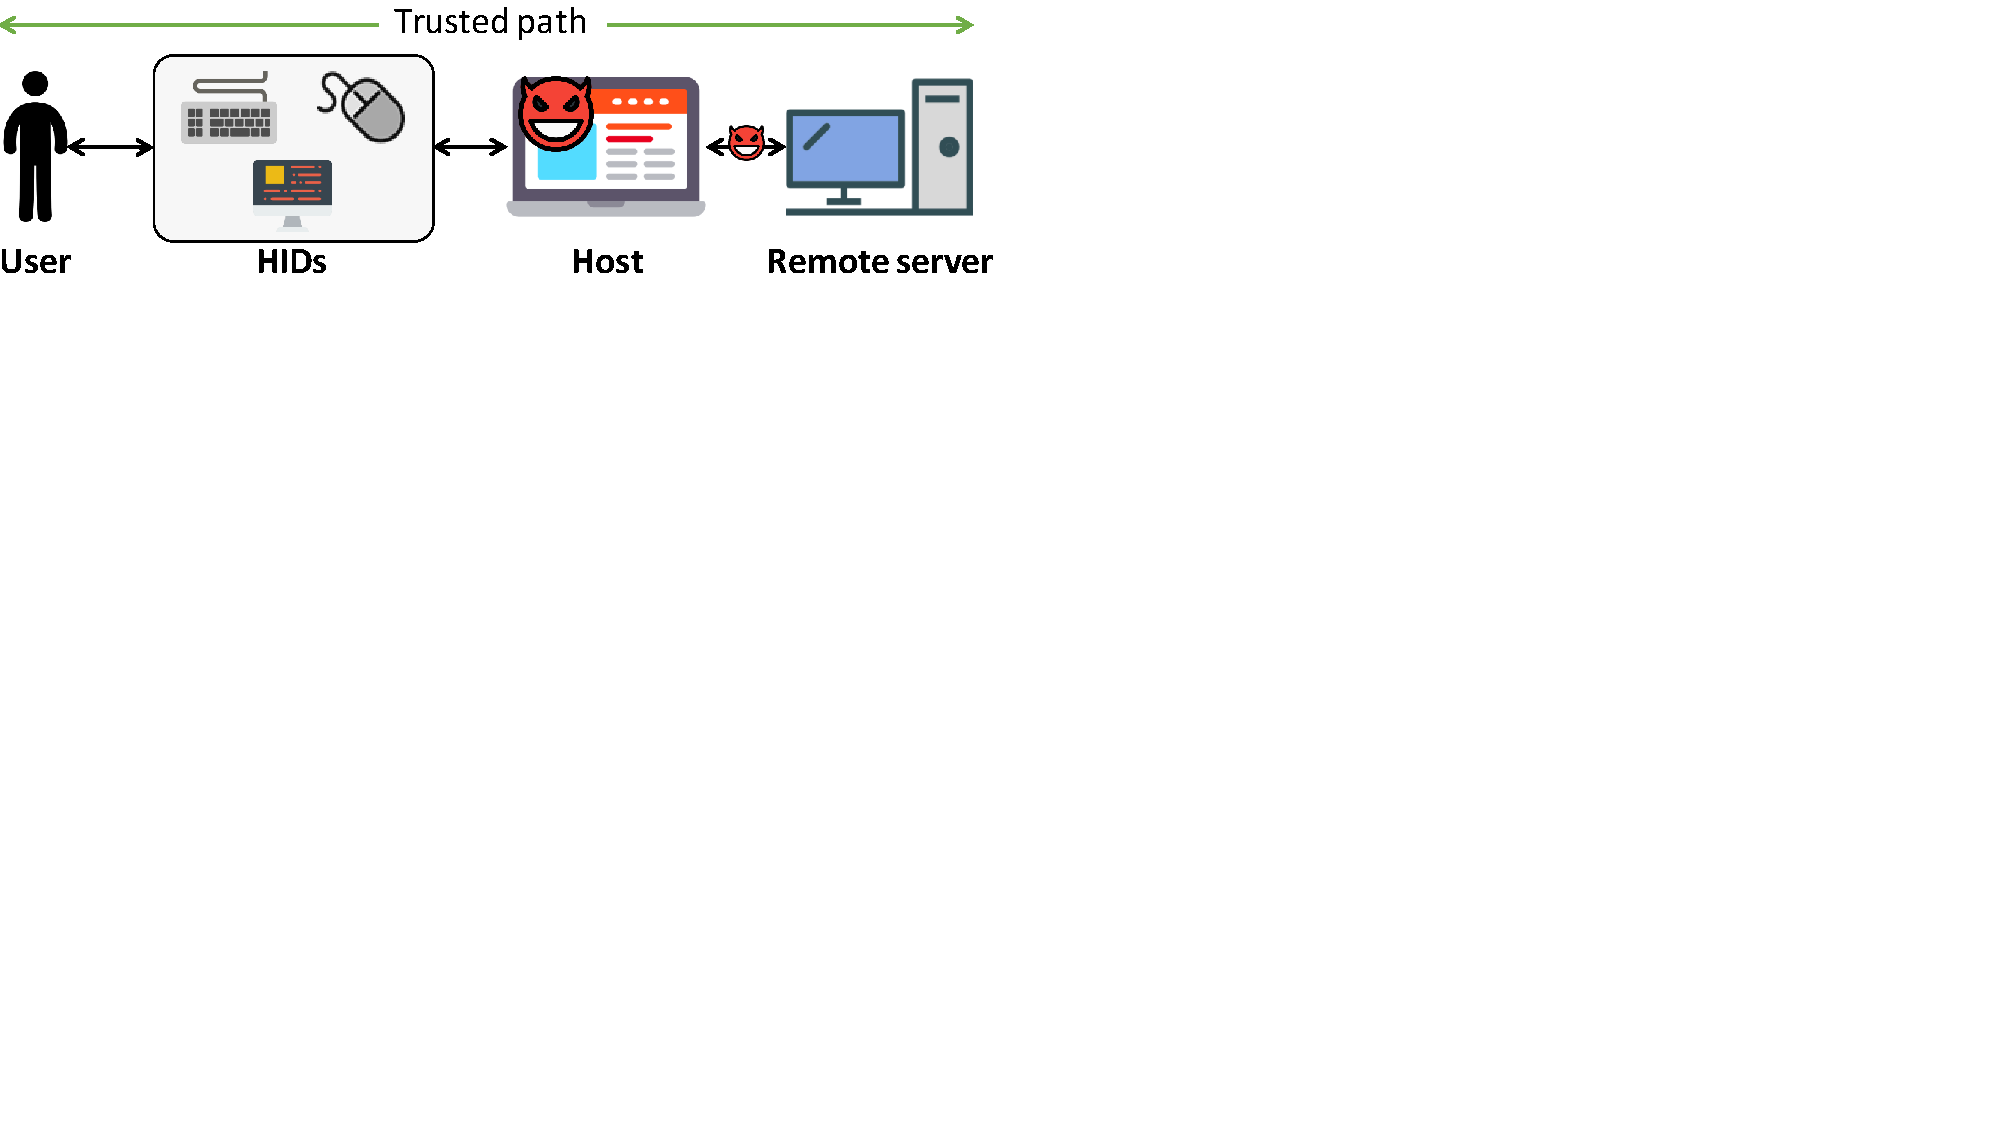
\includegraphics[trim={0 14cm 17cm 0}, clip, width=0.9\linewidth]{systemModel.pdf}
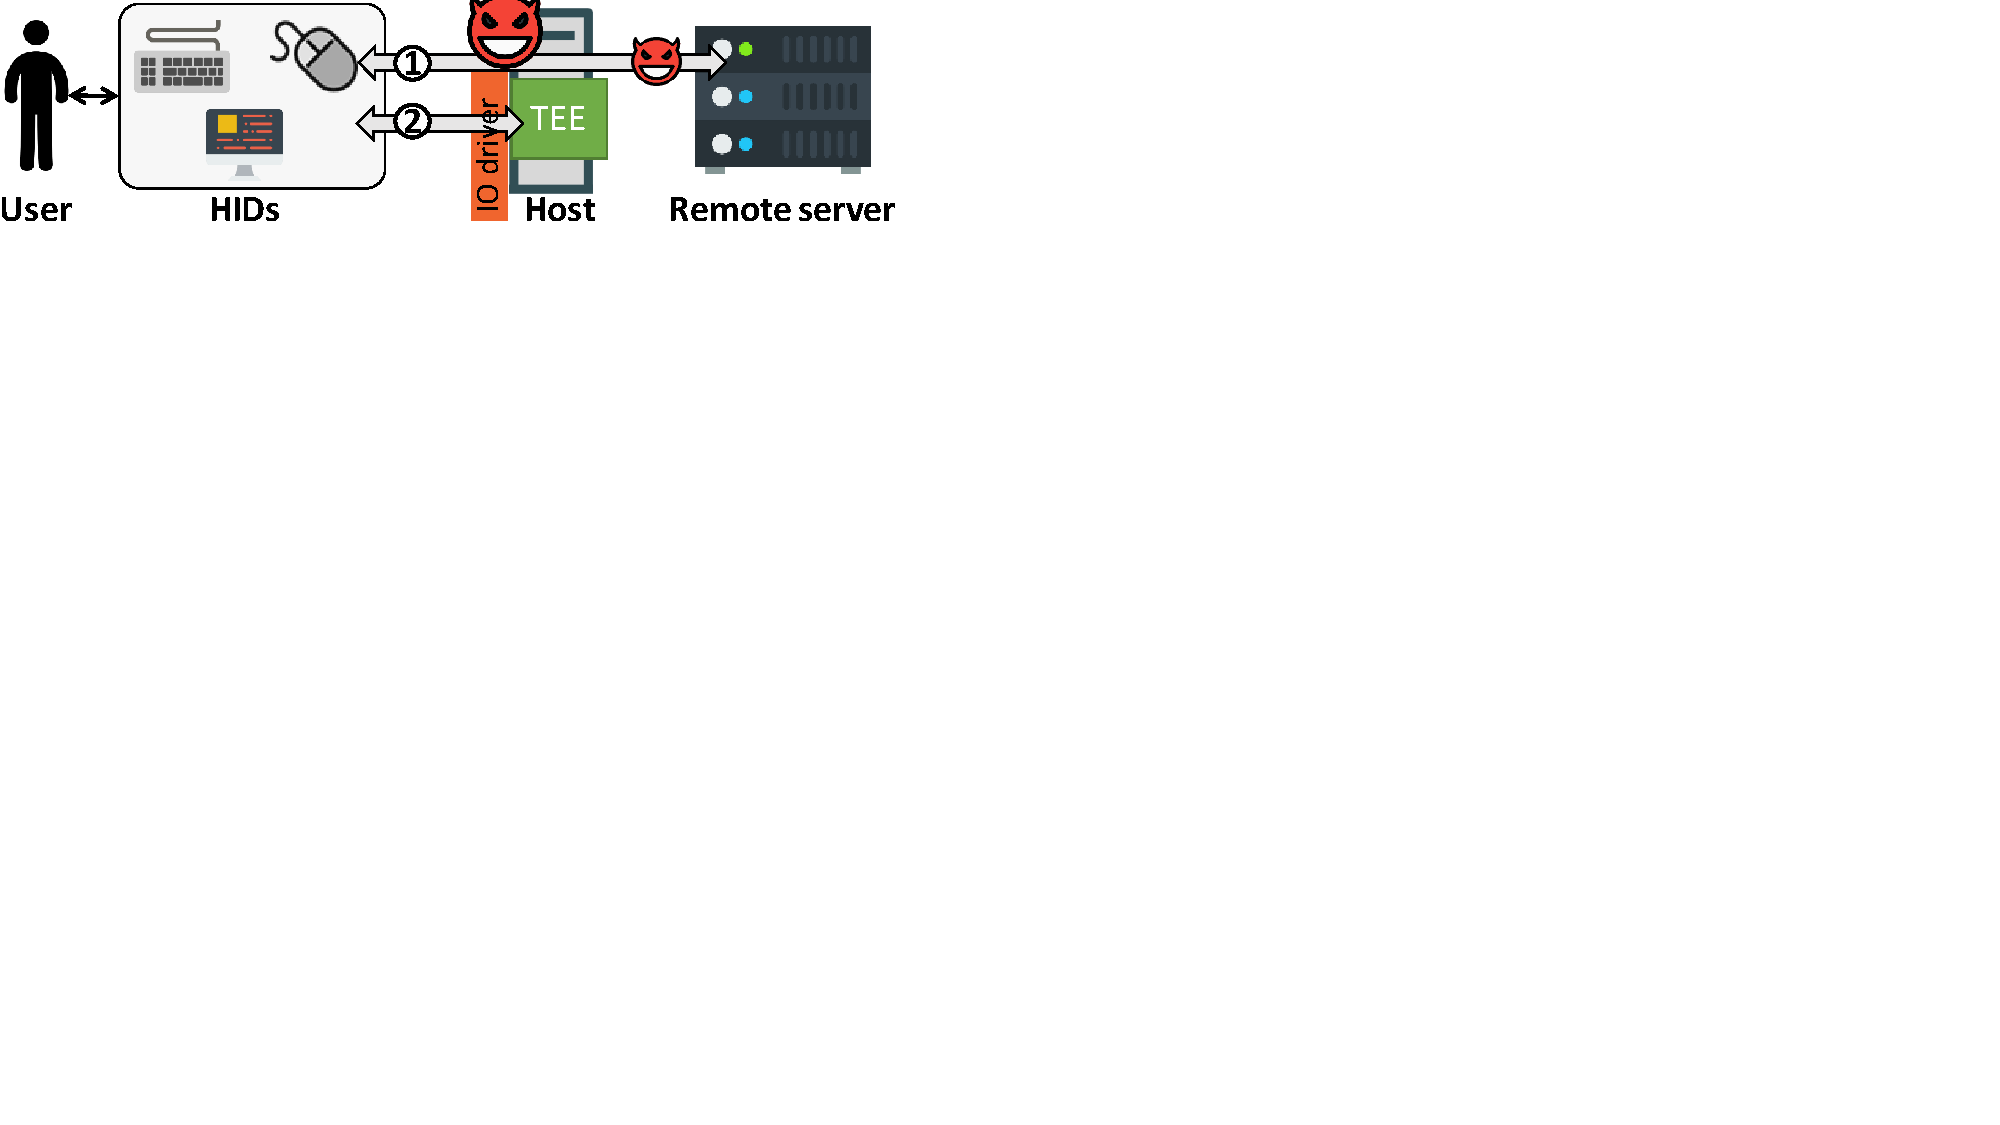
\includegraphics[trim={0 15cm 18cm 0}, clip, width=0.85\linewidth]{systemModel_all.pdf}
\caption{\textbf{Trusted path.} The figures shows the system and the attacker model of the trusted path. We generally consider two trusted path scenarios, \one trusted path to a remote server, and \two trusted path to a trusted execution environment (TEE) such as the Intel SGX.}
\spacesave
\label{fig:trustedPath}
\centering 
\end{figure}

In traditional settings, a \emph{Trusted path} provides a secure channel between the user and a trusted application running on the local host. The trusted path allows the user to ensure that her input reaches the intended application rather than a malicious one, and the output is generated by the legitimate application. However, in the setting where the local host is fully compromised, the trusted path to the local host is not possible as the trusted path requires a trusted endpoint, except if the local host supports TEE that runs in isolated enclaves. Establishing a trusted path to a remote server is non-trivial as the IO data is mediated by an untrusted operating system. Figure~\ref{fig:trustedPath} shows two different scenarios where the trusted path extends from user IO devices to \one a remote server, and \two a local enclave. %In principle, a trusted path solves the general security problem of the IO data. 
%But practically establishing a trusted path in general IO devices is a nontrivial problem specifically if one considers the plethora of complex UI objects and input methods as well as different security and functional properties that a solution should satisfy. 
In this paper, we primarily target the trusted path problem to a remote server (such as a remote PLC, web server or remotely accessible medical device, etc.) that is being accessed from a browser running on a commodity $x86$ host.


\myparagraph{Attacker model and capabilities} Our attacker model assumes that the host (OS, installed applications, and hardware) and the network are attacker-controlled. The attacker can intercept, drop, or modify the user IO data to and from the remote server. On top of it, the host can launch complex UI-based attacks. Such includes spawning multiple mouse pointer to trick the user into following the wrong mouse pointer and clicking on a wrong UI element, changing the layout of the UI elements (changing the position, size, adding, deleting or replacing UI elements, adding fraudulent instruction/information on the screen, changing labels of the UI elements, e.g., changing units of the input parameters, changing behaviour of the UI elements, etc.) to trick the user into providing sensitive data, manipulate input data, etc. 

\iffalse
\subsection{Security Properties}

A \emph{Trusted path} provides confidentiality and integrity to the IO data exchanged between the users and the end systems. In principle, a trusted path solve the general security problem of the IO data. But practically establishing a trusted path in general IO devices is a nontrivial problem specifically if one considers the plethora of complex UI objects and input methods as well as different security and functional properties that a solution should satisfy. We list these properties below. 


\begin{mylist}
  \item \textbf{Input integrity and confidentiality.} These properties define that any input that is coming from the user input devices are fully protected in two ways: i) the input issued by the user reaches to the remote end-point as it was generated by the user - \emph{integrity}, and ii) in specific application scenarios, the attacker-controlled host is entirely oblivious about the input from the user - \emph{confidentiality}. The trusted path system should consider a wide range of input devices, such as keyboard, mouse, touch, etc. We consider any sort of input action by the user that may include moving the mouse or using the keyboard navigation keys to select a specific item in a list.
  
  
  \item \textbf{Output integrity and confidentiality.} Similar to the input integrity, output integrity ensures that information that is sent by the remote endpoint is presented to the user as it was meant to be. One example of output integrity is the integrity of the UI elements. Such property ensures that the host system renders the UI elements faithfully as they were sent by the remote system. Output confidentiality ensures that the information sent by the remote server can not be accessed by the attacker-controlled host. 
  
 %  \item \textbf{Usability.} The trusted path should neither change the typical user interaction with a computer nor should require extensive changes into the existing systems.

  As discussed on the Section~\ref{sec:securityAnalysis}, ensuring output integrity is essential for providing input integrity against advanced attackers that trick the user into sending non-legitimate data to the server. For example, the user wants to send a number \texttt{10} to the server, but the malicious host shows on screen \texttt{100} and fools the user into believing he mistyped a \texttt{0}. The user deletes one \texttt{0} and sees \texttt{10} on the screen---as he intended initially---and submits the data, however, on the server arrives just \texttt{1}. 
  
  Providing output integrity is a challenging task even on systems that have a trusted component that overlays parts of the HDMI frames generated by the untrusted host. Previous works~\cite{huang2012clickjacking} show that when a trusted component and an untrusted one share a screen, the attacker can still manipulate the user to commit unintentional actions to the trusted UI if the system is not designed properly. In our solution, we want to guarantee that the user is aware of the UI elements (trusted or untrusted) that she interacts with, therefore preventing related attacks.
  \end{mylist}

\fi




\subsection{Existing and Strawman Solutions and their drawbacks}
\label{sec:problemStatement:existingSolution}

\iffalse
\begin{figure}[t]
\footnotesize
    \centering
    \begin{tikzpicture}[
solved/.style={rectangle,draw,fill=purple!40, rounded corners, align=center},
not/.style={rectangle, draw,fill=orange!60, rounded corners, align=center},
neutral/.style={rectangle, draw, rounded corners, align=center, fill=black!5}
]]
    \node[neutral](root) {Trusted path}
    child { node[neutral, yshift=12pt] (hw) {External\\ HW}}
    child { node[neutral, yshift=8pt, xshift=10pt] (tc) {Transaction\\ confirmation\\ Device}}  
    child { node[neutral, yshift=12pt, xshift=20pt] (tee) {TEE}
      child { node[neutral, yshift=0pt, xshift=-5pt] (teehv) {Hypervisor+\\TEE}}
      child { node[neutral, yshift=0pt, xshift=2pt] (teehw) {TEE + \\ External HW} } }
      child { node[neutral, yshift=8pt, xshift=15pt] (br) {Browser\\ Based}}   
     child { node[neutral, yshift=12pt, xshift=20pt] (hv) {Hypervisor}}  ;
    
    \node[below=0cm of hw] {\textbf{\name}};
    \node[below=0cm of tc] {Uni-dir~\cite{filyanov2011uni}};
    \node[below=0cm of hv] {Overshadow~\cite{Overshadow}};
    \node[below=0cm of teehv] {SGXIO~\cite{weiser2017sgxio}};
    \node[below=0cm of teehw] {Fidelius~\cite{Fidelius}};
     \node[below=0cm of br] {InContext~\cite{blake1998authenticated}};    
    \end{tikzpicture}
    
   \caption{\textbf{Summarization of existing trusted path solutions} by their approach. A detailed description of the related works is discussed in Table~\ref{tab:relatedWorks}.}
     \label{fig:relatedWorksTree}
\end{figure}
\fi





There are two broad categories of existing solutions that address the problem of trusted paths for IO devices in the presence of a compromised host as illustrated in Figure~\ref{fig:relatedWorksTree}: \textbf{A.}~Solutions where unprotected user interaction first happens and then a trusted component (transaction confirmation device) is used to double check that manipulation did not happen, and \textbf{B.}~Solutions where a trusted component captures user's input/output and then securely mediates them to the destination. The trusted component can be a browser, hypervisor, external hardware, etc. %But all of these solutions targeted for different problem settings and models. 
%Figure~\ref{fig:relatedWorksTree} provides a board classification of the related works and illustrates where our proposed work stands concerning them. %We can generally classify the work into two broad categories based on the trusted path approaches transaction confirmation device and existence of other trusted components.

\myparagraph{A.~Transaction confirmation devices} In their paper, Filyanov et. al~\cite{filyanov2011uni} proposed transaction confirmation device that requires the user to use a separate device to confirm the input parameters. Systems such as ZTIC~\cite{weigold2011secure} use an external device with display and smartcard attachment to ensure the integrity of the user inputs. Android OS also provides similar mechanism to confirm protected transactions~\cite{android_confirm}. 
However, these approaches suffer from three significant drawbacks: i) the risk of \emph{user habituation} -- users confirming transactions without looking to the actual data~\cite{anderson2016warning},
%Transaction confirmation devices introduce significant cognitive load to the user and may push the user to confirm their actions without even looking to the input data. 
ii) \emph{usability}, i.e., interacting with a small device can be cumbersome, iii) only \emph{simple UI} can be supported, i.e., transaction confirmation is not practical/suitable for complex interaction, rather simple text-based inputs.

%In contrary, \name supports generic input devices and supports complex user interfaces and user interactions. Moreover, the complete automated nature of \name does not introduce any cognitive load on the user, making the system less susceptible to user error.

\begin{figure}[t]
\scriptsize
    \centering
    \begin{tikzpicture}[
solved/.style={rectangle,draw,fill=purple!40, rounded corners, align=center},
not/.style={rectangle, fill=white, align=center},
neutral/.style={rectangle, draw, rounded corners, align=center, fill=black!5}
]]
  \node[not](empty) {};
    \node[neutral, right=3cm of empty](root) {Trusted path}
    child { node[neutral, yshift=10pt, xshift=-70pt, yshift=10pt] (tc) {\textbf{A.} Transaction\\ confirmation Device}}  
    child { node[neutral, yshift=10pt, xshift=10pt, yshift=15pt] (td) {\textbf{B.} Trusted intermediary}       
        %child { node[neutral, yshift=0pt, xshift=-30pt, yshift=7pt] (tee) {\textbf{B2.} TEE}}
      child { node[neutral, yshift=2pt, xshift=-50pt, yshift=7pt] (br) {\textbf{B1.} Browser-based}}   
     child { node[neutral, yshift=2pt, xshift=-25pt, yshift=7pt] (hv) {\textbf{B2.} Hypervisor-based}} 
     child { node[neutral, yshift=2pt, xshift=0pt, yshift=7pt] (hw) {\textbf{B3.} External HW}}
    } ; 
      

    \node[below=0cm of hw](gurdion) {\textbf{\name}};
    %\node[below=0cm of tee] {VButton~\cite{li2018vbutton}};
    \node[below=0cm of tc] {Uni-dir~\cite{filyanov2011uni}};
    \node[below=0cm of hv](os) {Overshadow~\cite{Overshadow}};
    \node[below=0cm of os] {SGXIO~\cite{weiser2017sgxio}};
    \node[below=0cm of gurdion] {Fidelius~\cite{Fidelius}};
     \node[below=0cm of br](ic) {InContext~\cite{blake1998authenticated}};
     \node[below=0cm of ic] {W3C UI security policy~\cite{w3c_spec}};

    
    \end{tikzpicture}
    
   \caption{\textbf{Existing trusted path solutions} by their approach. A detailed description of the related works is discussed in Table~\ref{tab:relatedWorks} in Appendix~\ref{appendix:summaryResearch}.\red{Todo: Update}}\spacesave
     \label{fig:relatedWorksTree}
\end{figure}

%None of these works looked into complex user interactions such as mouse movement or complex user interfaces. 


%\myparagraph{B2. Trusted Execution Environments} TEEs specifically system TEEs such as ARM TrustZone is used in the literature to implement a trusted path between the IO devices and the users. VButton~\cite{li2018vbutton} leverages ARM TrustZone to overlay buttons on the mobile device to confirm if the user taps on a specific button. Our solution is fundamentally different from VButtion as i) VButtion is specifically tuned for mobile devices, employing ARM TrustZone whereas our solution is more generic and targets specifically PCs, and ii) mouse input is significantly different than touch-based input as mouse input involves continuous movement where the touch or taps are discrete events. In this paper, we concentrate on the non-specialized hardware platform where compatible TEE technologies such as ARM TrustZone may not be available, e.g., x86 architecture. 
%Intel SGX based trusted path such as BastionSGX~\cite{BASTION-SGX} implements a trusted Bluetooth application inside an Intel SGX enclave to establish a trusted path between the keyboard and mouse and the SGX. But lack of output integrity makes the system unreliable as the paper failed to address how to transfer the mouse data reliably to the user and the remote server. 

%\myparagraph{B1. Browser-based solutions} InContext~\cite{huang2012clickjacking} presents different clickjacking attacks variants and their solution by ensuring context (both temporal and visual) and pointer integrity. Similarly, W3C UI security specification~\cite{w3c_spec} recommends developers to annotate the security-critical UIs in order for the browser to prevent malicious objects from being rendered on top of them.
%Clickjacking Revisited~\cite{akhawe2014clickjacking} evaluates such security measures in the context of a trusted browser. 

%\noindent\textbf{$\bullet$ Observations:} The browser-based solutions provide many useful techniques (details in Section~\ref{sec:systemDesign:userAttention}) to focus user attention to a sensitive UI. As our trust model assumes that the host is untrusted, adapting most of these technique is non-trivial.

\myparagraph{B1.~Trusted hypervisor-based solutions} Trusted hypervisors and secure micro-kernels are also alternatives to achieve Trusted path. In work done by Zhou et al.~\cite{zhou2012building}, the authors proposed a generic trusted path on $x86$ systems in pure hypervisor-based design. Solutions such as SGXIO~\cite{weiser2017sgxio}  combine a TEE and a hypervisor to mitigate the shortcomings of TEEs like SGX (the IO operations being handled by the OS).
Nevertheless, solutions based on hypervisors require a large TCB. 
%One major drawback of such solutions is the trust assumption that involves a full hypervisor. 
Formally verified hypervisors offer limited functionalities, therefore making them impractical for average users. One can argue that a hypervisor that provides a rich set of functionalities has a code size comparable to an actual OS. Also, systems employing TEEs such as Intel SGX open up new attack surfaces that can be exploited by microarchitectural attacks~\cite{van2018foreshadow}.

%There exist several works that use TEE and hypervisor simultaneously to mitigate the shortcomings of TEEs like SGX (i.e., the IO operations are handled by the OS). Existing research such as SGXIO~\cite{weiser2017sgxio} requires the IO drives to be implemented inside the TEE or using trusted hypervisor that extends the size of the TCB significantly. Moreover, TEE requires trust assumption on the processors and additional code bases. One such example is Intel SGX where the trust model includes the physical processor package, SGX SDK, quoting enclave, launch enclave and Intel attestation service. Our proposed solution avoids such extensive trust assumptions and assumes that the entire platform is in control of the attacker.

%Note that the majority of the previous works achieve some form of trusted path specifically for keyboard-based input. However supporting mouse and touch-based input, complex and generic user interfaces and protected users' action (such as the movement of the mouse pointer, gestures, etc.) in a security-sensitive application (such as e-voting) is not a trivial task. Without proper analysis of every frame that the host system produces, it is not possible to track user intention. In our knowledge, our proposed solution is the first to provide such security properties, including the confidentiality of user input (e.g., mouse movement). Moreover, we want to achieve this in the absence of any TEE as the trust model of our scenario is significantly different.

%Detailed description of the related research is described in Table~\ref{tab:relatedWorks} in Appendix~\ref{sec:summaryResearch}.
\myparagraph{B2. External hardware-based solutions} Several existing works propose a trusted path that utilizes an external trusted device. IntegriKey~\cite{IntegriKey} uses a trusted external device that contains a small program which signs all the user input and sends the signed input to the remote server. The device works as the second factor for input integrity as the remote server can verify if the signed input matched with the user input that is sent by the browser running on the untrusted host. However, as the external device is completely oblivious to the display information that the untrusted host renders, it is vulnerable UI manipulation attacks. For example, assume that the user's intended input to a textbox is $100$. She types the correct value but the host renders $10$ on the screen by not showing the last zero. Thinking that she may have mistyped, the user types another $0$ that makes the recorded input from the user $1000$. This attack violates input integrity as the host can now submit $1000$ to the remote server, and the external trusted device also signs $1000$ as the correct input received from the user.

\noindent\emph{$\rightarrow$ Observation 1:} The first observation is that the lack of output/visualization integrity compromises input integrity.

\begin{figure}[t]
\centering
%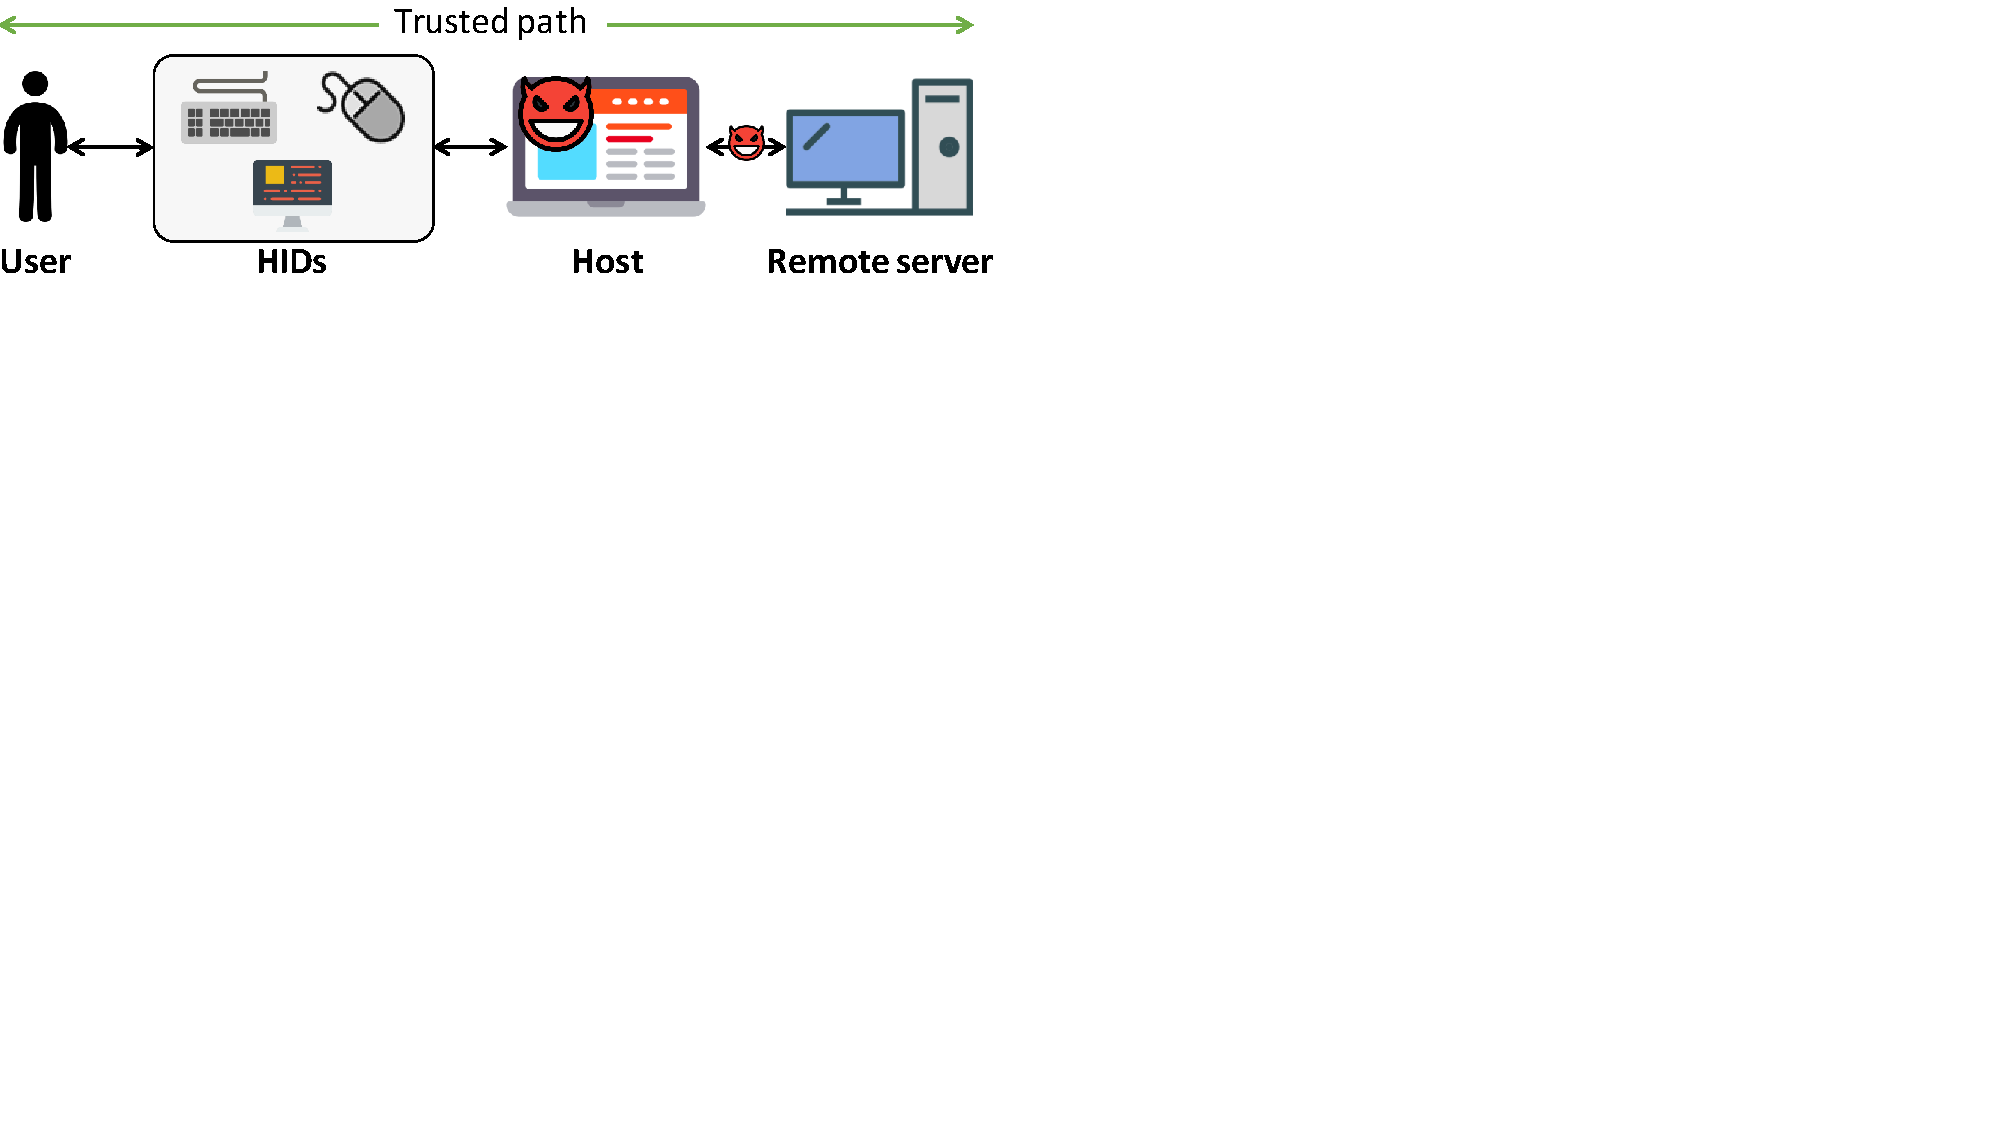
\includegraphics[trim={0 14cm 17cm 0}, clip, width=0.9\linewidth]{systemModel.pdf}
%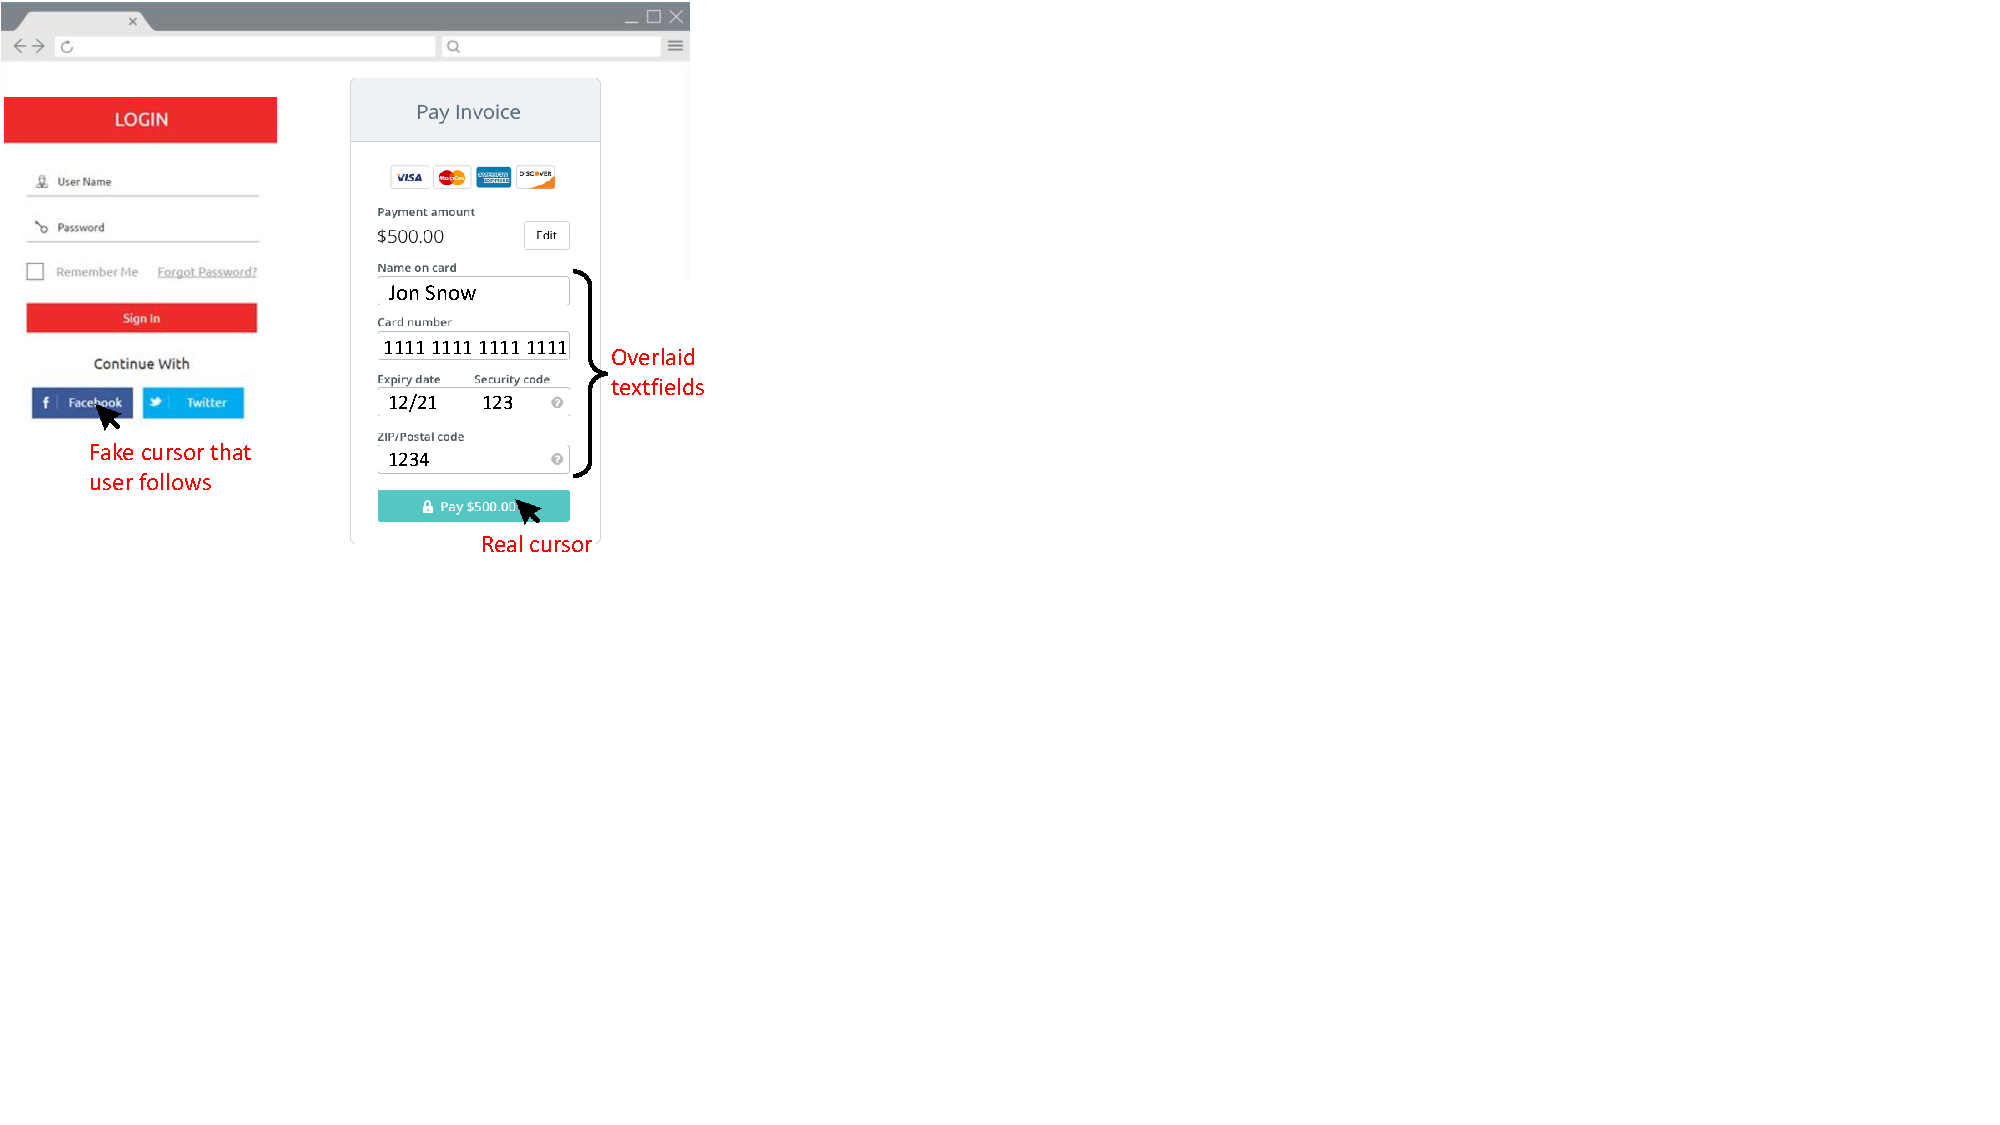
\includegraphics[trim={0 9cm 22cm 0}, clip, width=0.85\linewidth]{clickJacking.pdf}
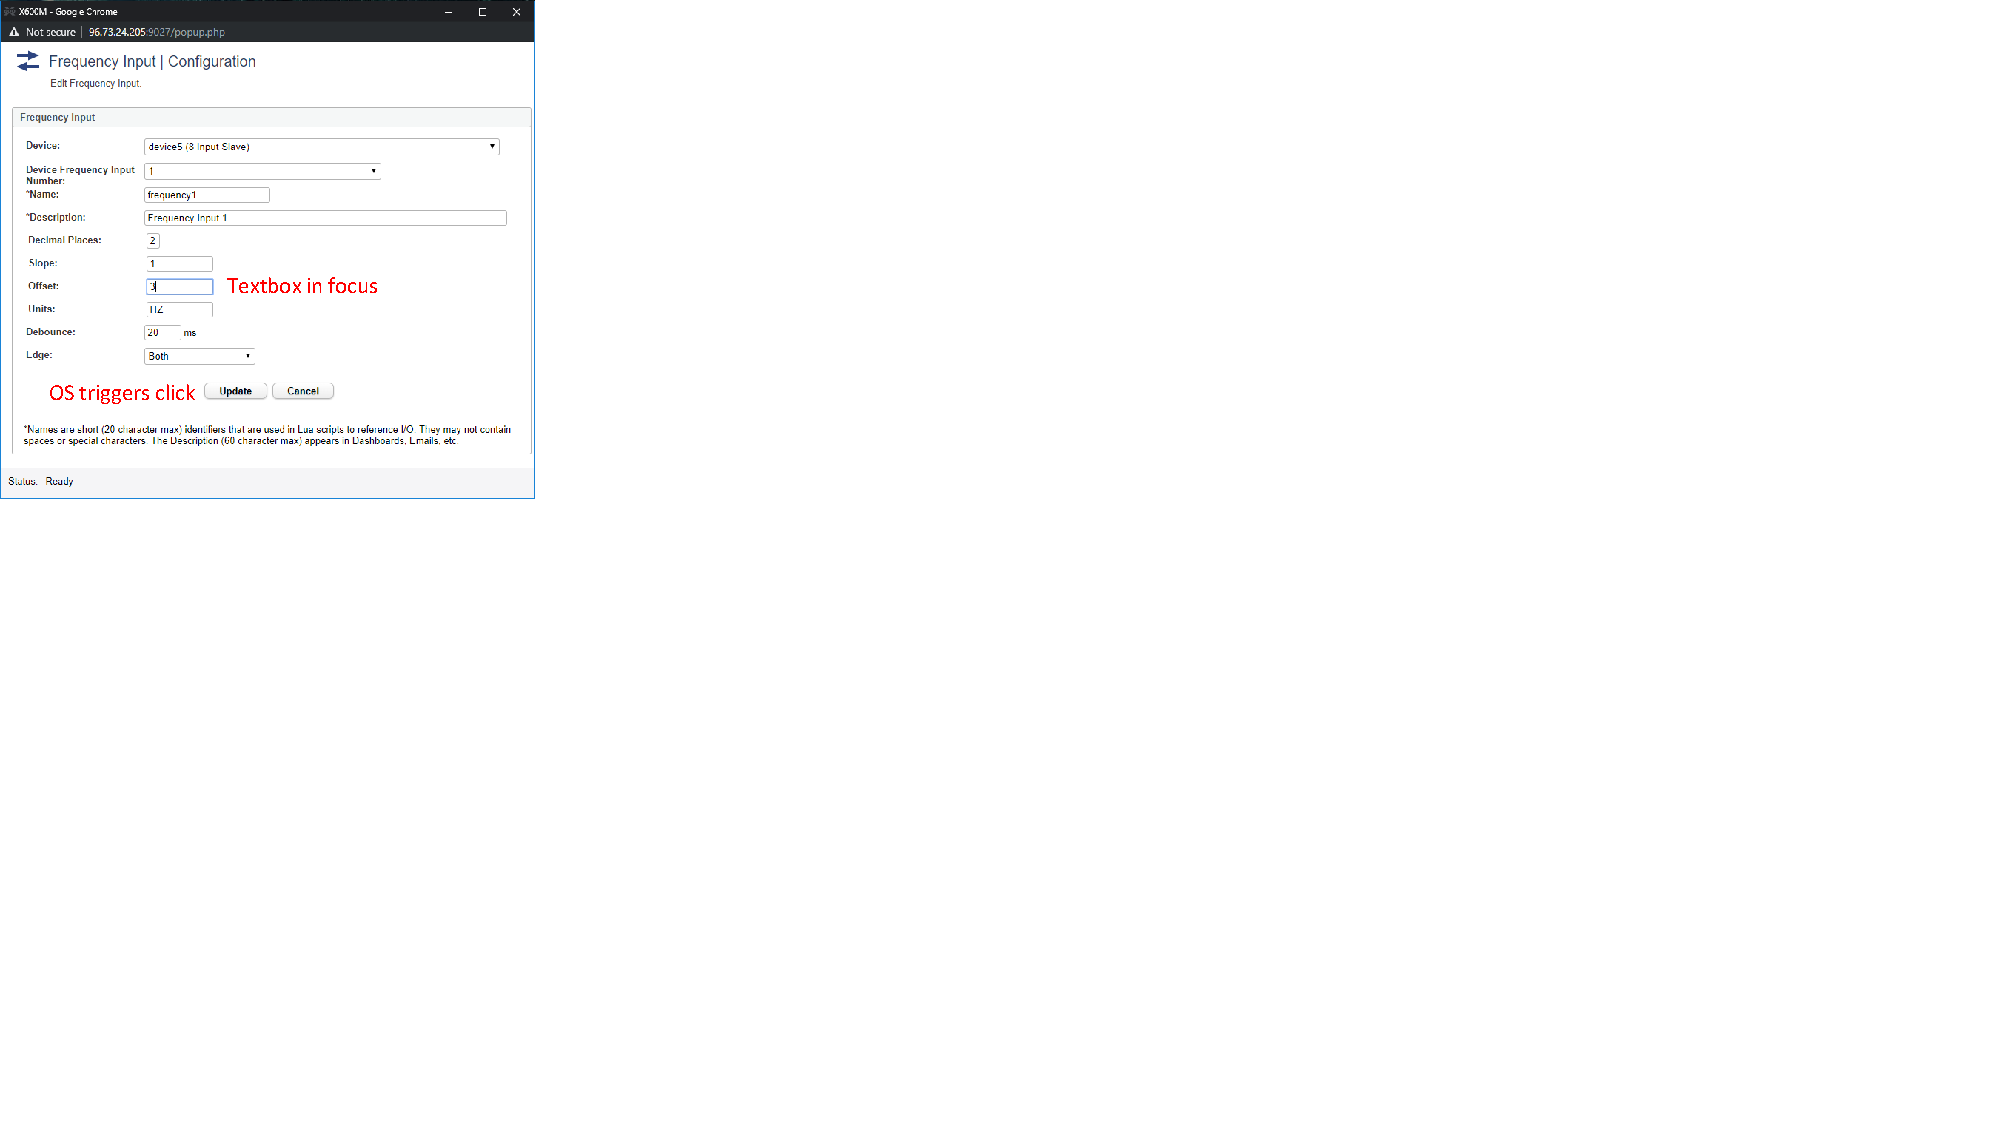
\includegraphics[trim={0 10.3cm 24.7cm 0}, clip, width=0.8\linewidth]{earlyFormSubmission.pdf} 
\caption{\textbf{Early form submission attack.} The figure shows an early form submission attack that Fidelius~\cite{Fidelius} is susceptible to. The user selects and edits the field \texttt{offset} while the OS triggers \texttt{Update} button, causing misconfiguration of a remote safety-critical PLC (screen shot is from a commercially available web-based PLC Control by Web X-600M~\cite{controlbyweb}).}
\spacesave
\label{fig:clickJack}
\centering 
\end{figure}


One of the recent solutions is Fidelius~\cite{Fidelius} which provides a more usable solution compared to previous ones. Fidelius uses an external trusted device and Intel SGX to create a secure channel between the user IO devices and a remote server. The device intercepts user keystrokes and does not deliver any event to the untrusted host when the user types to secured text fields. Additionally, Fidelius renders an overlay with the user inputs on the screen which is inaccessible by the host. This way, the untrusted host does not have access to the raw inputs and the user has a soft experience as her inputs are rendered on the screen as usual.
%provides secure input and display for the character-based device - keyboard. It uses overlays on the text fields to hide the keyboard input from the compromised host so that the input is only visible to the user. 
A small bar on display is also overlaid by the device that shows the remote server's identity and the text field that is currently selected. 
%However, Fidelius suffers from the following security and functionality issues: 

%Fidelius solely relies on the static overlay bar and the LEDs on the external device to ensure the integrity and confidentiality of the input. 
Fidelius introduces a high cognitive load to the users as they need to monitor multiple security indicators simultaneously before filling up one text field. Previous research works~\cite{egelman2008you,sobey2008exploring, anderson2016warning} have shown that systems that require users to observe multiple security indicators %that require the users to observe multiple markers on the screen (and also on an external device) 
do not guarantee security in practice.
Also, in specific scenarios the user training to properly explain these indicators could be a significant drawback for a real deployment.
%as the users require training to familiarize with the system (such as different security indicators).
Fidelius overlays only user inputs on the screen and keeps them isolated from the host. However, the rest of the screen is rendered by the untrusted host.
%the text fields and the character inputs into those text fields. 
This allows the attacker to modify the instructions on the UI, such as changing the unit of the input (described in the label of the text field) that result in an incorrect input.
%similar to the transaction confirmation devices (\textbf{A} in Figure~\ref{fig:relatedWorksTree}).  

\noindent\emph{$\rightarrow$ Observation 2:} The second observation is that if \emph{both output and input integrity} are not protected simultaneously, none of them can be achieved.

Fidelius does not support the integrity of the mouse pointer and its interaction with UI elements. The OS can arbitrarily trigger a mouse click on the submit button of the form and send incomplete data to the server - early form submission attack as illustrated in Figure~\ref{fig:clickJack}.
Moreover, Fidelius is vulnerable to clickjacking attacks where the attacker can spawn a fake mouse pointers and trick the user into following it while the real mouse pointer is on a sensitive text field protected by the system. This allows the attacker to fool the user into providing (possibly incorrect) input, while the user thinks that she is interacting with a non-sensitive text field. To prevent such attacks, the user has to look at the security indicators continuously even when she is not doing any security-sensitive task, which is a very strong assumption. 
Thus, not supporting the mouse causes the integrity violation of the keyboard input.

\noindent\emph{$\rightarrow$ Observation 3:} The third observation is that if not \emph{all the modalities of inputs} are secured simultaneously, none of them can be fully secured. 

Finally, the design of Fidelius is strictly limited to text-based fields only. As Fidelius does not provide output integrity of the forms, it cannot provide confidentiality to other UI elements such as radio buttons, drop-down menus, sliders, etc.
Microarchitectural attacks on Intel SGX increase significantly the attack surface of the system also~\cite{van2018foreshadow}.
%s such as Fidelius that rely on SGX for security against malicious OS and applications.

%\noindent\textbf{$\bullet$ Observation:} The main observation from the existing works concerning external devices are that i) \emph{lack of output integrity} compromises input integrity, ii) if \emph{both output and input integrity} are not protected simultaneously, not of them can be achieved, and iii) if not \emph{all the modalities of inputs} are secured simultaneously, none of them could be secure. 


%\myparagraph{Strawman solution I: Full-fledged isolated system} The first strawman solution uses an external trusted device that runs a full operating system with a browser and is physically isolated from the attacker-controlled host. From the security point of view, this solution does not provide any security benefits - the external device has the same attack surface as the untrusted host due to its huge TCB, making it as vulnerable as the host.

\myparagraph{Strawman solution I: Capturing screenshot} This strawman solution uses a trusted device that takes a screenshot when the user executes an action, e.g., mouse click to submit a form. The device then signs the snapshot and transmits it to the server along with the signed input. The remote server verifies the signature and then uses image/text analysis to extract the information from the UI elements such as labels on buttons or markers of a slider, etc. Therefore the server would detect if the host has manipulated UI elements when presented to the user.

This method is vulnerable to attacks because it does not capture spatio-temporal user context. This implies that the attacker may show some spacial information on the screen to influence the user that may not be captured by the snapshot\footnote{Taking full-screen snapshot could reveal also private information of the user from other applications visible on the screen.}. Similarly, taking a snapshot does not guarantee that a specific UI has been presented on the screen as the attacker may render the legitimate UI shortly before the device captures the snapshot.
One way to mitigate this problem is to capture a video of user interaction. But such a method requires the host to send large amounts of data to the server, and video processing is both time and CPU intensive. 
Lastly, adversarial machine learning techniques~\cite{eykholt2017robust,sitawarin2018rogue} make the image/text recognition techniques insecure against sophisticated adversaries.


\subsection{Requirements of Security Properties}
\label{sec:problemStatement:goals}

The lack of security properties and features in the existing solutions provides the necessary security requirements for IO integrity and confidentiality. We can not summarize the observations that we derived from the literature and the strawman solutions (refer to Section~\ref{sec:problemStatement:existingSolution}) as the following:


\begin{mylist}
  \item \textbf{Inter-dependency between input and output.} The main lessons that we learn from the previous papers are that input and output integrity, and confidentiality cannot be ensured in isolation. Rather, they are needed to be secured simultaneously as the output, and the input influences each other.  

  \item \textbf{Inter-dependency between all input modalities.} If there exist multiple input sources (typically keyboard and mouse), all of them are needed to be protected simultaneously as these input sources influence each other. For example, in web application scenario, protecting the integrity of only the keyboard input in does not provide any meaningful security in the web-application scenario as an attacker-controlled host can always execute an early form submission attack.

  
  \item \textbf{Low cognitive load for integrity.} Output integrity protection can eliminate the actions that leads to high cognitive loads to the user.  Such as using an external device to confirm every transaction, looking to a passive security indicator and confirming actions, etc. The systems that rely heavily on such security measures suffer from input errors that originate from user habituation. Moreover, such designs require heavy user training that makes the system deployment hard and costly.
  %Our goal is not to change the way users interact with UI elements and to impose no or minimal cognitive load such as eliminating the need to see an external device to confirm every transaction, looking to a passive security indicator and confirming actions, etc. The systems that rely heavily on such security measures suffer from input errors that originate from user habituation. Moreover, such designs require heavy user training that makes the system deployment hard and costly.
  
    %\item \textbf{Ease of deployment.} Our goal is also to provide a solution that comes with low deployment overhead such as eliminating any design choices that requires user training, a plug-and-play device that uses off-the-shelf components, the solution is compatible with any platform (OS, processor architecture, etc.), and does not require to install additional applications in the host.

  \item \textbf{Cognitive load for confidentiality.} Confidentiality requires active triggering from the user to distinguish the secure part of the screen from insuring part of the screen if the part of the output provides integrity/confidentiality protection.
  
  
  \item  \textbf{Small trust assumption.} Our goal is to provide the aforementioned rich set of IO and security features with minimal trust assumption that does not rely on a specialized hypervisor or a trusted OS  or TEEs such as Intel SGX. %Rather \name only trust a plug-and-play small-TCB trusted device that is made out of off-the-shelf components.  

\end{mylist}

%In the following section, what follows is the \name's design and how \name achieves these goals.
